%% LyX 2.3.6.1 created this file.  For more info, see http://www.lyx.org/.
%% Do not edit unless you really know what you are doing.
\documentclass[twoside,english]{report}
\usepackage[T1]{fontenc}
\usepackage[latin9]{inputenc}
\usepackage[a4paper]{geometry}
\geometry{verbose,tmargin=1in,bmargin=1in,lmargin=1.5in,rmargin=1in}
\setcounter{secnumdepth}{3}
\setcounter{tocdepth}{3}
\usepackage{babel}
\usepackage{array}
\usepackage{float}
\usepackage{booktabs}
\usepackage{graphicx}
\usepackage{nomencl}
% the following is useful when we have the old nomencl.sty package
\providecommand{\printnomenclature}{\printglossary}
\providecommand{\makenomenclature}{\makeglossary}
\makenomenclature
\usepackage[unicode=true,pdfusetitle,
 bookmarks=true,bookmarksnumbered=false,bookmarksopen=false,
 breaklinks=false,pdfborder={0 0 0},pdfborderstyle={},backref=false,colorlinks=false]
 {hyperref}

\makeatletter

%%%%%%%%%%%%%%%%%%%%%%%%%%%%%% LyX specific LaTeX commands.
%% Because html converters don't know tabularnewline
\providecommand{\tabularnewline}{\\}
\floatstyle{ruled}
\newfloat{algorithm}{tbp}{loa}[chapter]
\providecommand{\algorithmname}{Algorithm}
\floatname{algorithm}{\protect\algorithmname}

%%%%%%%%%%%%%%%%%%%%%%%%%%%%%% User specified LaTeX commands.
\pagenumbering{roman}
\usepackage{cite}
\usepackage[nottoc,notlof,notlot]{tocbibind}
\AtBeginDocument{\def\nomname{List of Abbreviations}}
\renewcommand{\nomgroup}[1]{%
\ifthenelse{\equal{#1}{A}}{\item[\textbf{Abbreviations}]}{%
\ifthenelse{\equal{#1}{B}}{\item[\textbf{Symbols}]}{%
\ifthenelse{\equal{#1}{C}}{\item[\textbf{Subscripts}]}
{}
}% matches Subscripts
}% matches Symbols
}% matches Abbreviations
\usepackage{algorithm,algpseudocode}

\makeatother

\def\eqdeclaration#1{, see equation\nobreakspace(#1)}
\def\pagedeclaration#1{, page\nobreakspace#1}
\def\nomname{Nomenclature}

\begin{document}
\title{RDMA over Converged Ethernet}
\author{Sherif Badran, Rami Rasheedi, Zeyad Madbouly, et al.\\
Computer and Systems Department\\
Faculty of Engineering, Ain Shams University\\
Cairo, Egypt}

\maketitle
\newpage{}
\begin{center}
\includegraphics[scale=0.1]{\string"images/ASU FOE LOGO\string".png}
\par\end{center}

\begin{center}
Ain Shams University, Faculty of Engineering
\par\end{center}

\begin{center}
Electronics and Communications Engineering Department
\par\end{center}

\begin{center}
Cairo, Egypt
\par\end{center}

\vfill{}

\begin{center}
\textbf{\Large{}RDMA over Converged Ethernet}{\Large\par}
\par\end{center}

\begin{center}
{\large{}A Report Submitted in Partial Fulfillment of the Requirements
of the Degree of Bachelor of Science in Electronics and Communications
Engineering }\textbf{\large{}\vfill{}
}{\large\par}
\par\end{center}

\begin{center}
By
\par\end{center}

\begin{center}
\begin{tabular}{lr}
\textbf{Mohammed Hussien Mostafa} & \textbf{1601160}\tabularnewline
\textbf{Mohamed khaled Mohamed Sayed El khawas } & \textbf{1601173}\tabularnewline
\textbf{Christine Magdy Gad El-Rab Samuel } & \textbf{16E0129}\tabularnewline
\textbf{Martina Fadi Fouad farag } & \textbf{1601053}\tabularnewline
\textbf{Maryham melad Gerges Michael } & \textbf{1601075}\tabularnewline
\end{tabular}
\par\end{center}

\begin{center}
\vfill{}
\par\end{center}

\begin{center}
Supervised by
\par\end{center}

\begin{center}
\textbf{Prof. Dr. Victor Goraldiz}
\par\end{center}

\begin{center}
Cairo 2021
\par\end{center}

\thispagestyle{empty}

\newpage{}

\chapter*{Declaration}

We hereby certify that this project submitted as part of our partial
fulfillment of BSc in Electronics and Communications Engineering is
entirely our own work, that we have exercised reasonable care to ensure
its originality, and does not to the best of our knowledge breach
any copyrighted materials, and have not been taken from the work of
others and to the extent that such work has been cited and acknowledged
within the text of our work.

Signed
\begin{center}
\begin{tabular}{l>{\centering}p{3cm}}
\toprule 
Name & Signature\tabularnewline
\textbf{Mohammed Hussien Mostafa} & \tabularnewline
\textbf{Mohamed khaled Mohamed Sayed El khawas } & \tabularnewline
\textbf{Christine Magdy Gad El-Rab Samuel } & \tabularnewline
\textbf{Martina Fadi Fouad farag } & \tabularnewline
\textbf{Maryham melad Gerges Michael } & \tabularnewline
\bottomrule
\end{tabular}
\par\end{center}

Date: Day of 24\textsuperscript{th} of July, in the year 2021.

\thispagestyle{empty}

\newpage{}

\chapter*{Acknowledgments}

Thank and acknowledge your advisor, family and friends.

\thispagestyle{empty}\newpage{}
\begin{abstract}
Nowadays, data have become a crucial aspect of all evolving computer
technologies. That\textquoteright s why owning data and knowing how
to use it efficiently has become a key of success to any enterprise.
Not only is data a crucial aspect of our modern life, but also the
speed at which applications are running and data can be accessed has
a significant impact as well. However, massive amounts of data that
need to be analyzed, processed, shared, transferred, monitored and
accessed (Big data/parallel computing/Cloud computing) have led to
very high work load on data centers and systems. This has led to slower
processing speeds and increased latency in response to user requests
or operations running. In addition, the high availability requirement
of any database has become exceedingly important and backup systems
are taken into consideration from the very beginning at the phase
of designing the system to ensure no or minimum down time and continuous
functionality. 

Our project proposes a methodology to tackle the above problems where
applications can directly access the memory and perform I/O operations
without CPU interference through DMA directly. Hence, minimizing latency
and maximizing the CPU processing speed. 

RDMA allows direct access of memory of one computer into the other\textquoteright s
memory without involving any OS. This is very useful nowadays in the
distributed systems where individual computers are connected together
and are communicating together easily to facilitate efficient data
transfer and parallel processing and resource sharing to appear as
one integrated system.

There are various RDMA protocols such as RoCE V.1 and RoCE V.2 and
IWARP. Ethernet is an alternative RDMA offering that is more complex
and unable to achieve the same level of performance as RoCE-based
solutions.

However, in our project, we have implemented RoCE V.1. RoCE is a network
protocol which allows accessing memory directly over an Ethernet network.
This is done through the encapsulation of IB transport packet over
Ethernet. 
\end{abstract}
\newpage{}

\tableofcontents{}

\newpage{}

\listoffigures
\newpage{}

\listoftables

\newpage{}

\listof{algorithm}{List of Algorithms}
\newpage{}

\printnomenclature[3cm]{}

\newpage{}

\nomenclature[A]{RDMA}{Remote Direct Memory Access}\nomenclature[A]{RoCE}{RDMA over Converged Ethernet}\nomenclature[A]{iWARP}{Internet wide-Area Network}\nomenclature[A]{NIC}{Network Interface Card}\nomenclature[A]{HCA}{Host Channel Adapter}\nomenclature[A]{API}{Apllication Programming Interface}\nomenclature[A]{QP}{Queue Pair}\nomenclature[A]{WOE}{Work Queue Element}\nomenclature[A]{CQE}{Completion Queue Element}\nomenclature[A]{HPC}{High Performance Computing}\nomenclature[A]{IETF}{Internet Engineering Task Force}\nomenclature[A]{RoCE V.1}{RDMA over Converged Ethernet version 1}\nomenclature[A]{RoCE V.2}{Routable RoCE}\nomenclature[A]{CPU}{Central Processing Unit}\nomenclature[A]{OS}{Operating System}\nomenclature[A]{RLDP}{Row Locality based Drain Plicy}\nomenclature[A]{DRAM}{Dynamic Random Access Memory}\nomenclature[A]{FCFS}{First come, First served}\nomenclature[A]{FR-FCFS}{First ready-First come, First served}\nomenclature[A]{LWM}{Low watermark}\nomenclature[A]{HWM}{High watermark}\nomenclature[A]{DDR}{Double Data Rate}\nomenclature[A]{FSM}{Finite State Machine}

\pagenumbering{arabic}
\setcounter{page}{1}

\chapter{Introduction}

\section{Introduction}

\section{Problem Statement}

\section{Objective}

\section{Outline}

\begin{algorithm}
\caption{Anything}

\begin{algorithmic}[1]
\Require{$\rho \geq 1$}
\Ensure{$X_k$}
\While{not converged}
\State{Solve $X_{k+1}=\min_{X} L(X,Y_k, \mu_k)$}
\State{$Y_{k+1}=Y_k+\mu_k h(X_{k+1})$}
\State{$\mu_{k+1}=\rho \mu_k$}
\EndWhile
\end{algorithmic}
\end{algorithm}


\chapter{Introduction to Virtual PCIe}

\chapter{Linux Kernel}

\chapter{Introduction to Memory systems}

\chapter{DDR5 Memory New Features}

\chapter{DDR5 Controller Architecture}

\section{Front-end }

\section{Back-end}

\chapter{DDR5 Controller Specifications}

\section{Address Mapping Scheme}

\section{Memory requests scheduling}

DRAM is the most commonly used technology for building memory systems.
However, it has been a main performance bottleneck for modern computer
systems. Hence, many request scheduling algorithms are designed in
order to reduce latency and exploit maximum row buffer locality. Exploiting
row buffer locality in DRAM is a main key characteristic while designing
proper scheduling algorithm for application needs. DRAM architecture
is segmented into multiple banks to support concurrent accesses. Each
DRAM bank consists of rows and columns of DRAM cells. Each bank is
accessible with a row buffer, accessing it is faster than accessing
different row in the same bank\cite{RLDP}.

We will discuss the main scheduling algorithms we studied during designing
phase:
\begin{enumerate}
\item FCFS 
\item FR-FCFS
\item RLDP 
\item Thread-Fair Request Reordering
\end{enumerate}

\subsection{FCFS }

\section{Bank Arbitration }

\subsection{Idea Behind Arbiter Design}

Before we discuss in such a deep way into design, we should show some
important timing constraints in the new DDR5 technology. First, 

Our proposed controller arbitration criteria aims to exploit maximum
concurrent processess supported by DDR5 bank groups technology, thus,
our arbiter is aiming to grant access to controller data path to new
bank groups if there are ready requests in it, Hence, exploiting maximum
available concurrent accessing into a DDR5 chip.

Choosing suitable arbitration sequence is so critical in order to
increase or performance. 

There are three timing constrains we should take into consideration
in the new DDR5 technology:
\begin{itemize}
\item Short access timing between two different bank groups:
\end{itemize}
Arbiter must take in consideration this constrain, whatever the current
group is, arbiter should select new different group to drain from.
\begin{itemize}
\item Long access timing between two different banks in the same bank group
and worst access timing between different rows in same bank:
\end{itemize}
Arbiter should choose different banks in same group before trying
to give access to same last bank in order to avoid row conflicts as
possible.

\subsection{Block Diagram}

hi iam block diagram

\begin{figure}
\noindent \begin{centering}
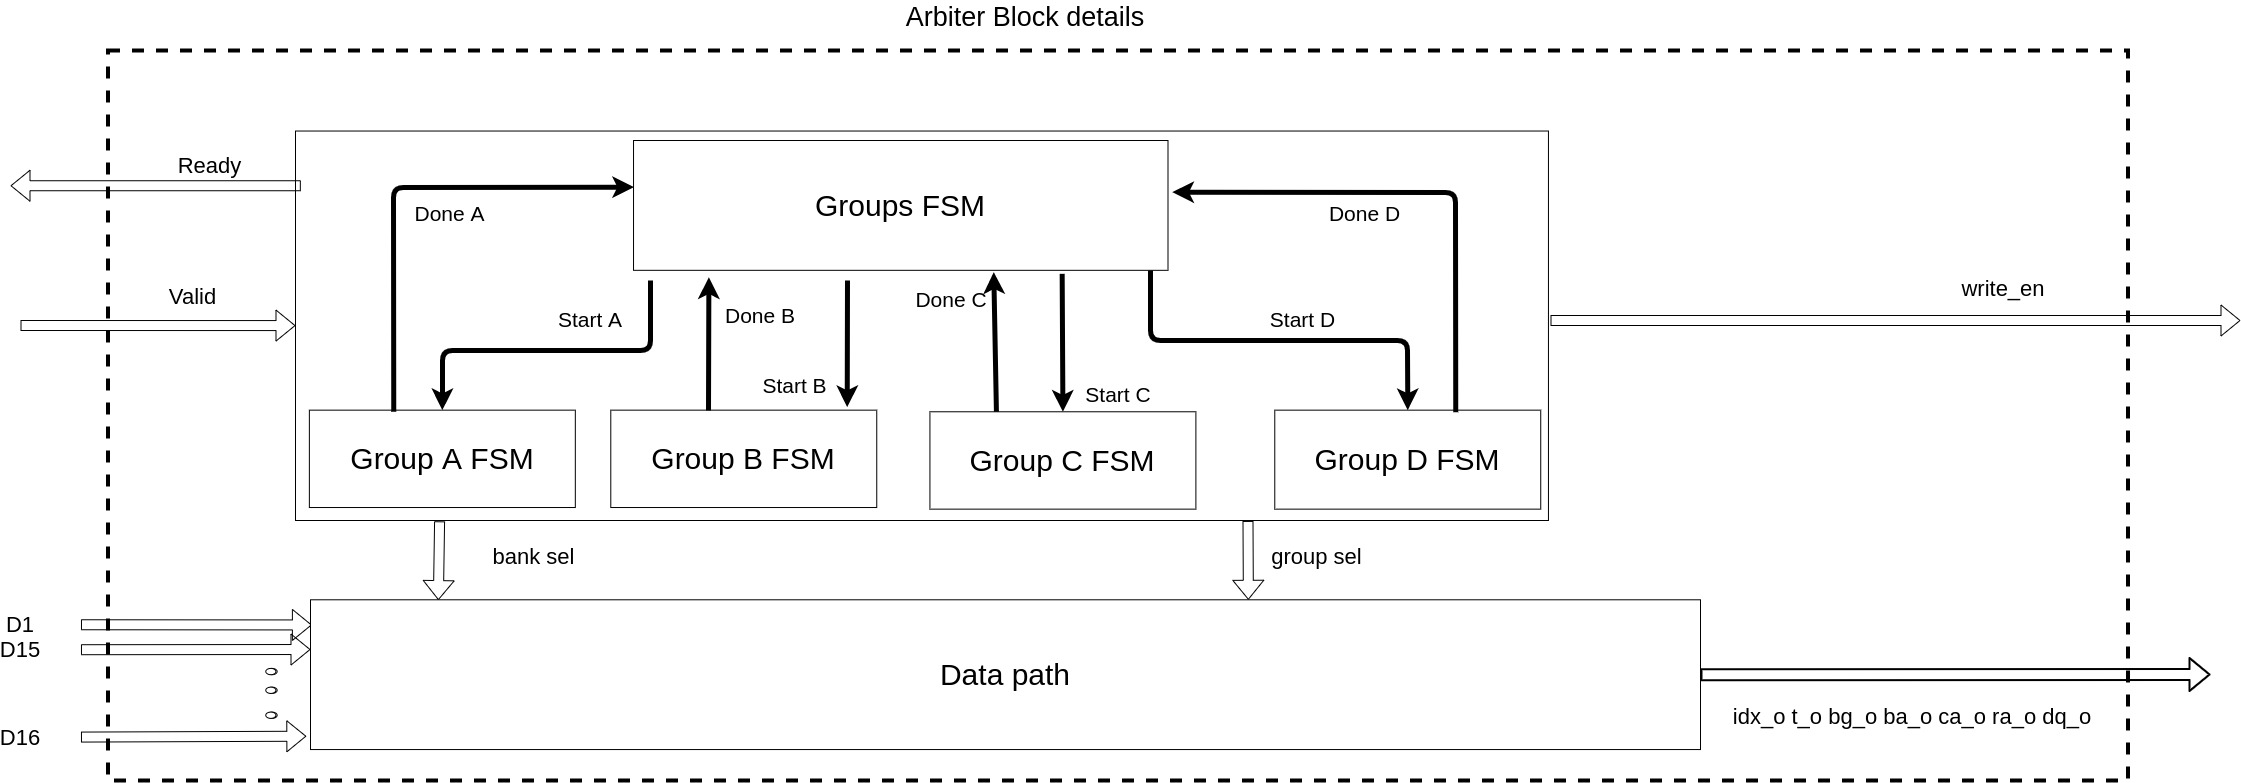
\includegraphics[viewport=0bp 0bp 2241bp 783bp,scale=0.15]{images/Arbiter_block_diagram}
\par\end{centering}
\caption{Arbiter block diagram}

\end{figure}


\chapter{Emulation Results\cite{Memorysystems,hdlchipdesign}\cite{mauerer2010professional}}

\begin{tabular}{|c|c|c|c|c|c|}
\hline 
edgdf &  & gfgf &  &  & fgfgfg\tabularnewline
\hline 
dfgd &  & dfgf &  &  & fgdggfgdg\tabularnewline
\hline 
fgf &  & gfgf &  &  & gfgf\tabularnewline
\hline 
 &  & gf & fg &  & gf\tabularnewline
\hline 
fgf &  & gfg &  &  & \tabularnewline
\hline 
\end{tabular}

\chapter{Conclusions and Future Work}

\bibliographystyle{IEEEtran}
\bibliography{Bibtex/generic_database}


\appendix

\chapter{First Appendix}

\chapter{Second Appendix}
\end{document}
